\section{Introducción}
\begin{frame}{Introducción - Historia de las matemáticas}
\begin{teor}
Cada entero positivo tiene una única descomposición en números primos.
\end{teor}
\end{frame}
\begin{frame}{Introducción - Complejidad algorítmica}
\begin{table}[H]
    \centering
    \begin{tabular}{lll}
        \hline
        Notación & Nombre & Ejemplo de algoritmo \\
        \hline
        $O(1)$ & Constante & Acceso a un elemento de un vector\\ 
        $O(log N)$ & Logarítmica& Búsqueda binaria\\
        $O(N)$ & Lineal & Búsqueda secuencial\\
        $O(N log N)$ & Lineal-Logarítmica& Algoritmo de ordenamiento \textit{quicksort}\\
        $O(N^2)$ &Cuadrática & Algoritmo de ordenamiento simple\\
        $O(N^3)$ &Cúbica & Multiplicación de matrices\\
        $O(2^N)$ &Exponencial & Partición de conjuntos\\ \hline
    \end{tabular}
    \caption{Ejemplos de algoritmos numéricos con su clasificación $O$ de complejidad}
    \label{tabla:notacion-O}
\end{table}
\end{frame}
\begin{frame}{Introducción - Complejidad algorítmica}
\center{Complejidad algortímica del algoritmo Criba General del Cuerpo de Números.}
\begin{equation}
    O\left(exp\left[c n^{1/3} \left(log n\right)^{2/3} \right] \right)
    \label{eq:O(clasico)}
\end{equation}
\end{frame}
\begin{frame}{Introducción - Origen de la computación cuántica}
\begin{tesis}[de Church]
    La clase de las funciones que pueden ser calculadas mediante un algoritmo coincide con la clase de las funciones recursivas.
\end{tesis}
\begin{tesis}[de Turing]
    La clase de las funciones que pueden ser calculadas mediante un método definido coincide con la clase de las funciones calculables mediante una Máquina de Turing.
\end{tesis}
\end{frame}
\begin{frame}{Introducción - Algoritmo de Shor}
    \center{Complejidad algorítmica del algoritmo de Shor}
    \begin{equation}
    O(n^2(logn)(log(logn)))
    \label{eq:compledidad_cuantica}
\end{equation}
\end{frame}
\begin{frame}{Introducción - Qiskit-IBM}
    \begin{figure}[H]
    \begin{subfigure}{0.4\textwidth}
        \centering
        \caption{}
    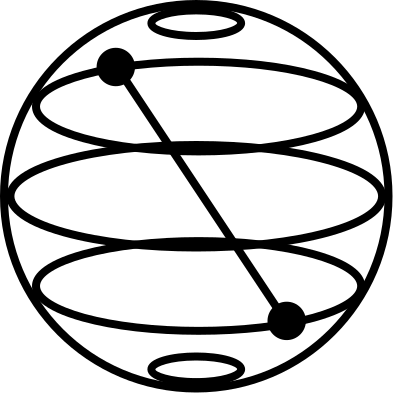
\includegraphics[height=4.5cm]{images/Qiskit.png}
    \label{fig:logo_qiskit}
    \end{subfigure}
    \begin{subfigure}{0.4\textwidth}
        \centering
        \caption{}
    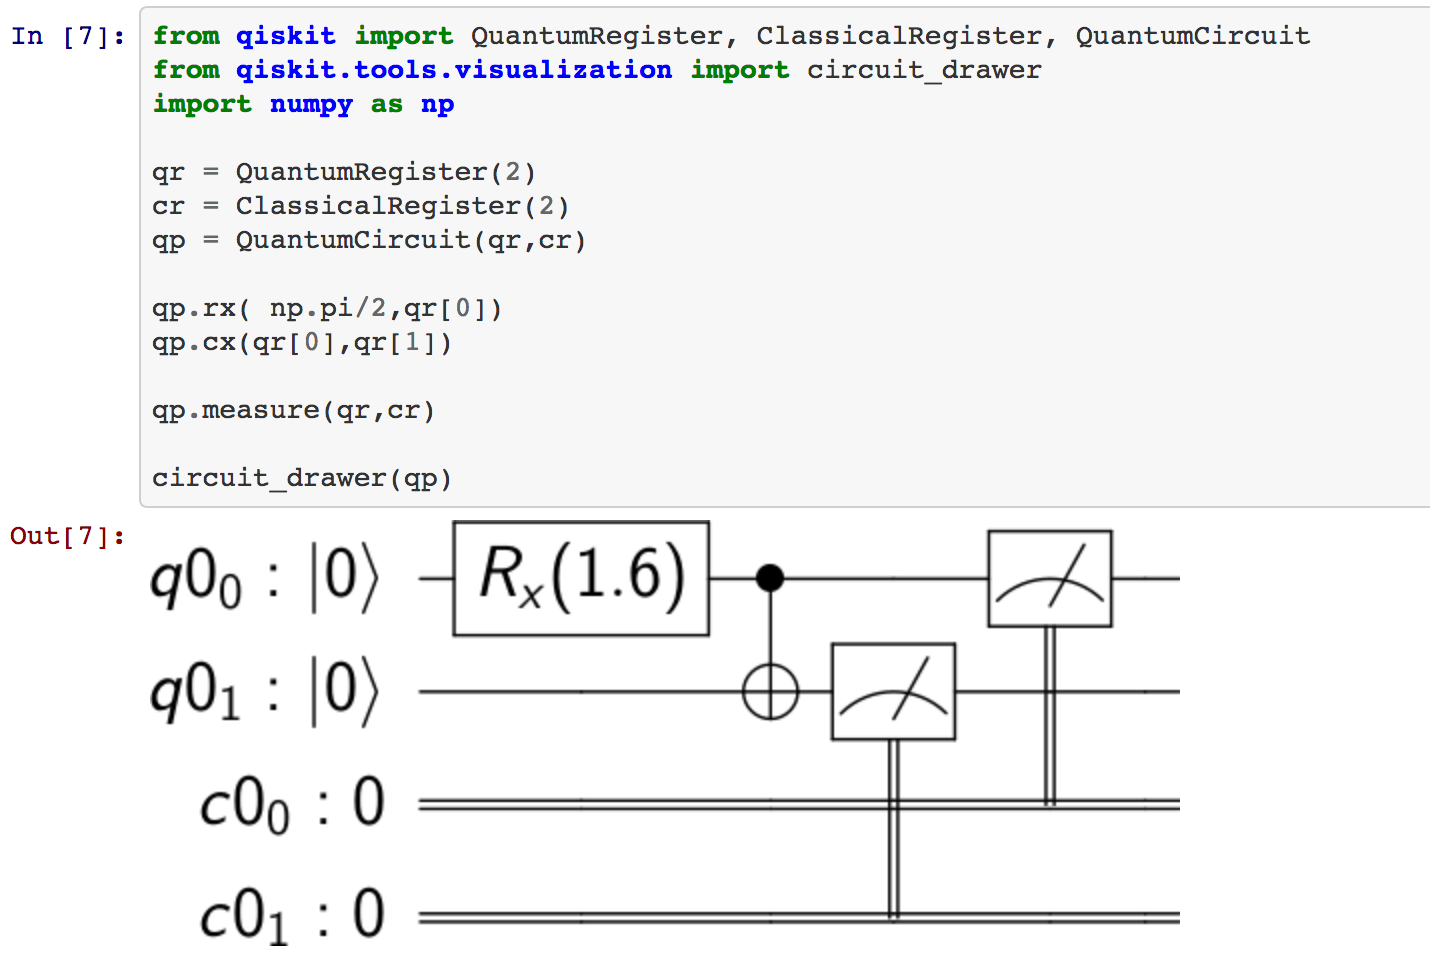
\includegraphics[height=5cm]{images/Example_qiskit.png}
    \label{fig:example_qiskit}
    \end{subfigure}
    \caption{(a) Logo de Qiskit, (b) Ejemplo de un circuito cuántico implementado dentro de Jupyter Notebook de Python.}
\end{figure}
\end{frame}